% !TeX root=../main.tex
\chapter{اجرای برنامه}
\section{پیشگفتار} 
در این فصل تلاش میشود که شیوه اجرا برنامه و خروجی گرفتن از آن توضیح داده شود؛
لازم به یادآوریست همانطور که در پیشنهاده آمده است تمرکز این پروژه طراحی یک اپلیکیشن نیست و هدف تنها ارائه یک مدل ریاضی برای مدار های الکتریکی می باشد، همچنین به همین دلیل محیط
\lr{google colab}
برای تست کردن مدل انتخاب شده است.
\section{مخزن پروژه}
تمام برنامه ها و اسناد موجود برای این پروژه از طریق آدرس 
\href{https://github.com/Mehrdadghassabi/Gracc}{پیوند}
شده قابل دسترسی است، همچنین در فایل
\lr{README.md}
توضیحات کوتاهی در مورد شیوه اجرا داده شده است، که البته در این فصل به توضیحات بیشتری پرداخته خواهد شد.
\section{یافتن خودکار پاسخ مدار}
\label{section:atm}
نمونه
\ref{section:ex1}
را در نظر بگیرید، میخواهیم پاسخ این مدار را به کمک برنامه نوشته شده بدست بیاوریم؛
نخست بایستی کتابخانه ای که نوشته شده را توسط دستور
\lr{pip install Gracc
}
\footnote{
	\lr{Gracc}
	نام پروژه حاضر است که خود مخفف واژه های
	\lr{Graph}
	و
	\lr{circuit}
	است.
}
نصب کنیم.
سپس بایستی به گونه ای یک مدار الکتریکی را به عنوان ورودی به حل کننده بدهیم؛
برای اینکار تصمیم گرفته شده است که مدار الکتریکی به شکل یک متن توصیف شود و آن متن به عنوان ورودی به حل کننده داده شود.

شیوه اینکار بدین صورت است که در خط اول
\lr{n}
که تعداد راس هاست و با یک فاصله
\lr{m}
که تعداد یال هاست نوشته میشود.و در
\lr{m}
خط بعدی شیوه اتصال راس ها می آید بدین گونه که
\lr{x y z a b c}
نمایانگر این است که راس شماره
\lr{x}
و راس شماره
\lr{y}
به یکدیگر متصل اند؛ و در بین آنها یک
مقاومت 
\lr{z}
اهمی،
یک باتری
\lr{a}
ولتی،
یک خازن
\lr{b}
فارادی
و یک سلف
\lr{c}
هنری موجود است؛
در صورت عدم وجود یکی از عناصر یک شده به جای مقدار آن صفر گذاشته و درصورت وجود چندین عنصر از یک نوع معادل آن را قرار میدهیم.

مدار
\ref{fig:fig4}
و گراف کیرشهف آن
\ref{fig:fig5}
را در نظر بگیرید، میخواهیم این مدار را به صورت متن توصیف کنیم؛
آشکار است که این گراف شش راس و هشت یال دارد و مثلا بین یال شماره صفر
\footnote{
	به صورت دلخواه شماره گذاری کنید!!
}
که 
\lr{A}
باشد
و یال شماره سه که
\lr{D}
باشد مسیری موجود است و آن مسیر دارای یک مقاومت ده اهمی و یک باتری بیست ولتی است؛
در نظر داشته باشید چون در گراف کیرشهف این مدار
\ref{fig:fig5}
مسیر از
\lr{A}
به
\lr{D}
در نظر گرفته شده و سمت منفی باتری بدین سو است بایستی مقدار آن منفی بیست ولت درج شود؛
اگر برای همه یال ها این روند را تکرار کنیم توصیف متنی این مدار بدین صورت
\ref{fig:fig7}
میشود
:
\begin{figure}[ht]
	\centerline{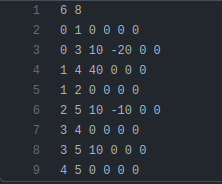
\includegraphics[width=9cm]{fig7}}
	\caption{توصیف متنی مدار
		\ref{fig:fig4}
	}
	\label{fig:fig7}
\end{figure}
پس از توصیف متنی مدار بدین صورت
\ref{fig:fig7}
آنرا اجرا کرده و جواب را می یابیم.
\begin{figure}[ht]
	\centerline{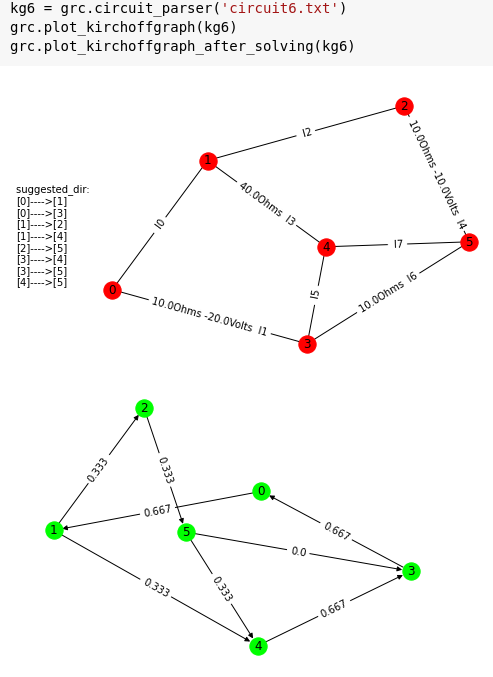
\includegraphics[width=9cm]{fig8}}
	\caption{جواب
		\lr{Gracc}
		برای مدار
		\ref{fig:fig4}
	}
	\label{fig:fig8}
	
\end{figure}
جواب نهایی در شکل 
\ref{fig:fig8}
آمده است.
\footnote{
	گراف بالایی خود مدار و پایینی جواب آن است
}
میتوانید آن را با جوابی که در
\ref{fig:fig5}
به صورت دستی بدست آوردیم مقایسه کرده و از درستی جواب اطمینان حاصل کنید.